\documentclass[twocolumn, german]{tum-article}

\usepackage{booktabs}
\usepackage{enumitem}
\usepackage[ngerman]{varioref}
\usepackage{graphicx}
\usepackage{xcolor}
%\usepackage{microtype} maybe

\usepackage[backend=biber,style=numeric,sorting=none]{biblatex}
\bibliography{literature_link.bib}

\title{{\color{TUMBlau} Maschinen- und Roboterethik:}\\Die komplexe Ethik autonomer Kraftfahrzeuge}
\author{Florian Schmidt\authormark{1, \,\Letter}}
\titlerunning{Ethik des autonomen Fahrens}
\authorrunning{Florian Schmidt}
\affil[1]{Fakultät für Informatik, Technische Universität München (TUM),
  Boltzmannstr. 3, 85748 Garching, Germany}
\email{fs.schmidt@tum.de}
\date{\today}

\begin{document}

\maketitle

Das autonome Fahren ist eine sehr gegenwärtige wissenschaftliche, wie technische Errungenschaft, die verspricht, innerhalb der nächsten Dekaden den Straßenverkehr umfassend zu revolutionieren. Am Horizont stehen in diesem Kontext selbst- und leer fahrende geteilte Fahrzeuge im Rahmen eines modernisierten Carsharings, die innerhalb von Großstädten maßgeblich zur Entzerrung der fahrzeuggefüllten Innenstädten beitragen können -- und auf dem Land selbstredend auch die Verkehrsinfrastruktur ausbauen könnten.

Bis entsprechende Fahrzeuge allerdings vollständig autonom auf den Straßen dieser Welt unterwegs sein können, sind allerdings noch einige Fragen offen. Fragen, auf die es möglicherweise auch keine schwarz-weißen, generalisierbaren Antworten geben könnte -- ja womöglich auch nicht geben kann. Fragen, die ethisch und moralisch höchst prekäre Entscheidungen einer algorithmisch denkenden oder künstlich intelligenten Maschine abverlangen, die den Kontext der Situation womöglich gar nicht verstehen kann. Fragen, denen sich die Gesellschaft früher oder später stellen muss, und für die im besten Fall eine globale Lösung gefunden werden könnte.

Die folgenden Überlegungen beschäftigen sich vorrangig mit ebendiesen ethischen Überlegungen des autonomen Fahrens.


\section{Grobeinordnung in die Maschinenethik}
Zu Beginn des Artikels wollen wir uns grundlegend mit der Maschinenethik beschäftigen, um die vorliegende Spezialisierung in den richtigen Kontext einzuordnen.


\subsection{Definition und Abgrenzung}
Grundsätzlich beschäftigt sich die Maschinenethik als solches mit den Konzepten der maschinellen Moral beziehungsweise der moralischen Maschine -- also mit der Überlegung, wie das doch relativ abstrakte Konzept der Moral mit der konkreten, technischen Maschine in Einklang zu bringen ist.

Kern der Überlegung ist ein naheliegender Gedanke: Mit der Forschung auf dem Gebiet der künstlichen Intelligenz werden technische Systeme geschaffen, die Anzeichen von Intelligenz nachweisen (sollen). Ist eine Maschine nun derart intelligent, liegt es dementsprechend auch nahe, dass sie auch Anzeichen von einer Moralvorstellung aufweisen könnte \cite[S. 3f.]{bendel-mascheth}.

Es zeigt sich, dass die beiden Phänomene der Intelligenz sowie der Moral zwar per se unabhängig sind, aber in ihrer Existenz dennoch korrelieren (siehe Abbildung \vref{fig:moral-ethics}). Ähnlich verhält es sich auch mit den Disziplinen der Maschinenethik und der Forschung an der künstlichen Intelligenz. Genauso wie die Maschinenethik an moralischen Maschinen forscht, versucht die Gegenseite künstlich intelligente Systeme zu erschaffen.

\begin{figure*}
	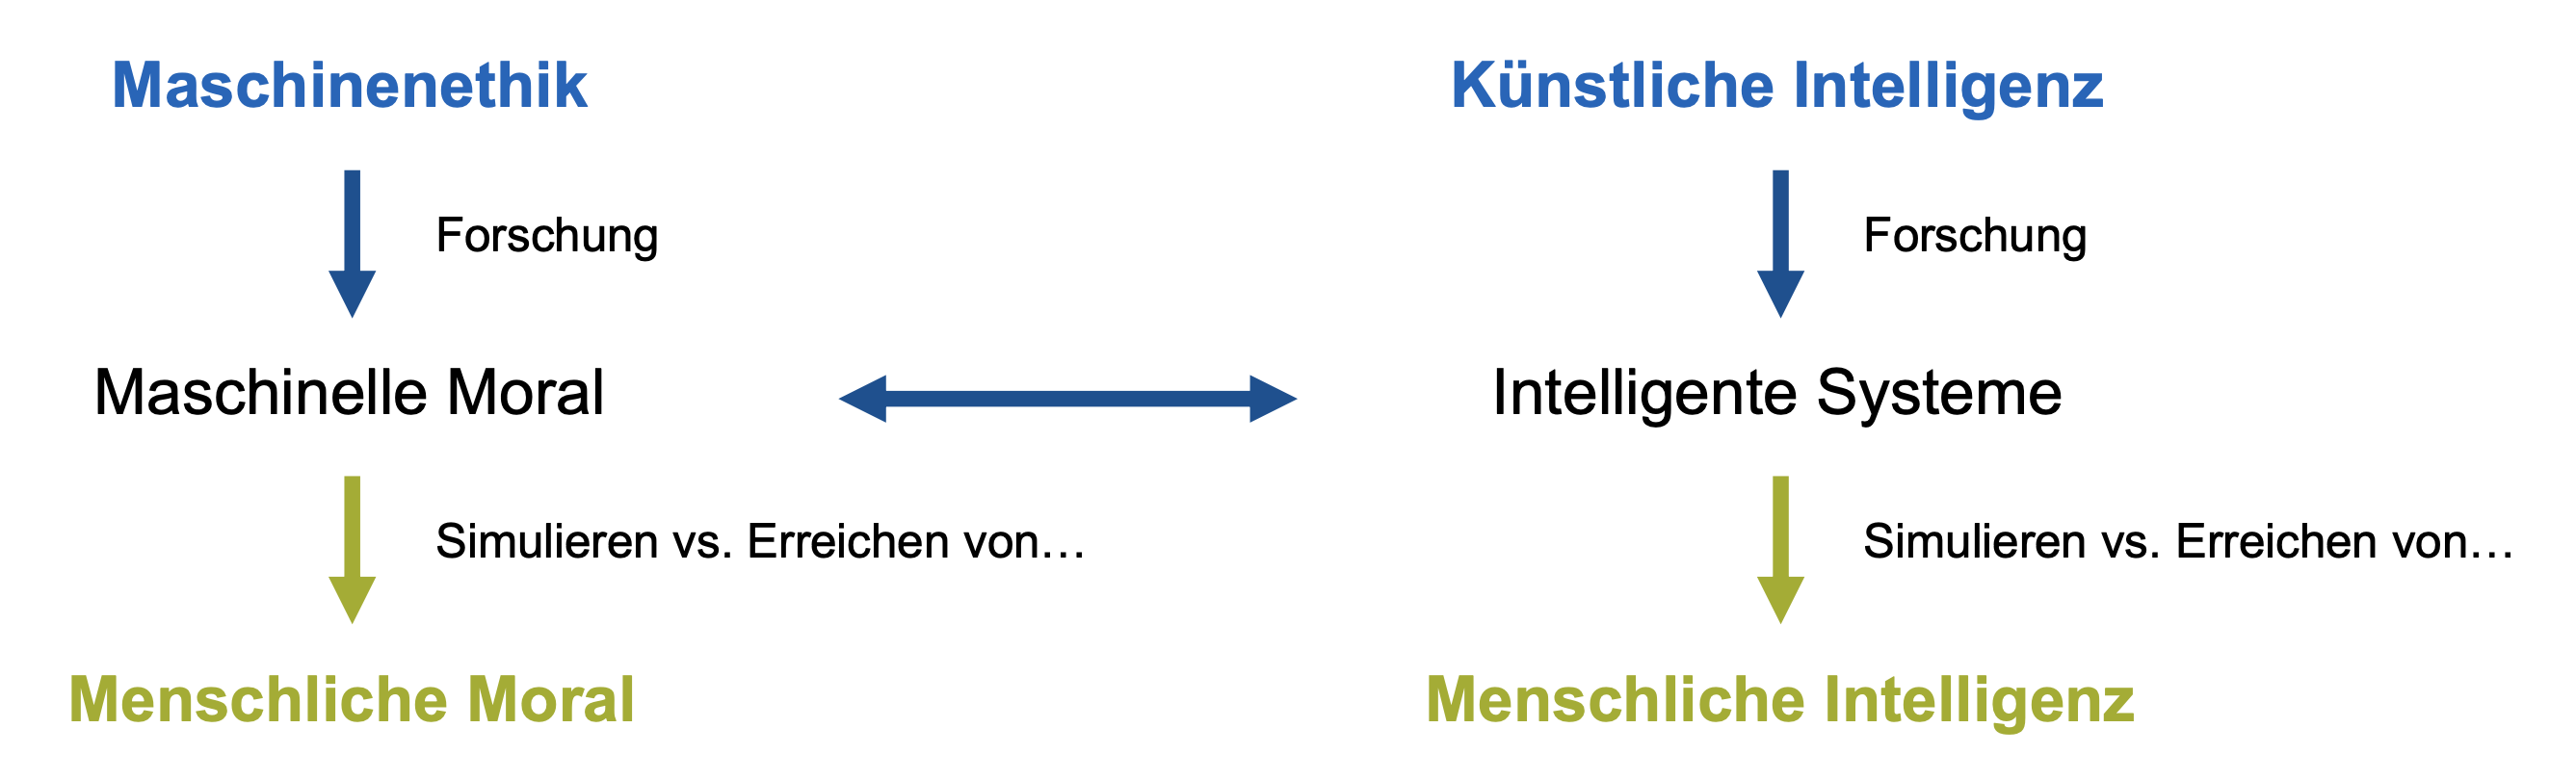
\includegraphics[width=\textwidth]{media/eth-int}
	\caption{Begriffliche Abgrenzung der maschinellen Moral und künstlichen Intelligenz \cite[S. 17]{bendel-mascheth}.}
	\label{fig:moral-ethics}
\end{figure*}

Analog kann man die Differenzierung zwischen der schwachen und starken Eigenschaft von der Forschung zur künstlichen Intelligenz übernehmen. Wir sprechen von schwacher maschineller Moral wie schwacher KI, wenn die entsprechende Eigenschaft simuliert oder in Teilen dem Vorbild nachgeahmt wird; erst die starke KI oder starke maschinelle Moral strebt danach, die Eigenschaft vollständig zu erreichen \cite[S. 17]{bendel-mascheth}. Die starke KI stellt hiermit also eine Art \emph{allgemeine} künstliche Intelligenz dar -- spätestens hier sind Überlegungen zur Moral in jedem Fall angebracht\footnote{Offen bleibt natürlich die Frage, ob die menschliche Moral in diesem Kontext das erstrebenswerte Ziel ist. Es kann ebenso Ziel sein, eine Art \glqq Moral\grqq{} zu erzeugen, die sich gänzlich von der des Menschen unterscheidet \cite[S. 23]{bendel-mascheth}.}.

Abgegrenzt wird die Maschinenethik in der Regel von den mit ihr verwandten Bereichsethiken
\begin{itemize}
	\item der \textbf{digitalen Ethik}, die sich im Kern mit informationstechnologischen Systemen und den damit einhergehenden Überlegungen zu informationeller Autonomie auseinandersetzt, sowie
	\item der \textbf{Technikethik}, die sich allgemeiner gefasst mit technischen und wissenschaftlichen Entwicklungen beschäftigt und ebendiese mit ethischen Wertungen versieht.
\end{itemize}


\subsection{Kernfragen}
Die zentrale Idee der Maschinenethik ist also, die Maschine also als Subjekt und nicht nur als Objekt der Moral zu sehen -- sprich die Maschine im Sinne der Moral auf eine dem Menschen gleichgestellte Ebene zu heben.

Die Notwendigkeit dieser Überlegungen ergibt sich direkt aus der wachsenden Autonomie der Maschinen. Trifft eine Maschine Entscheidungen, die ohne Zutun eines Menschen erfolgen, ist die Moral automatisch relevant. Erst recht gilt dies, sofern dieser Maschine eine Entscheidungsgewalt über Leben und Tod zusteht.

Evident ist, dass für diese Art von extremer Entscheidungsfindung ein gewisses Verständnis des Kontext der Handlung nötig ist. Konzepte wie Leben und Tod, Bewusstsein und Menschenwürde sind schwierig in imperative Programmzeilen zu encodieren -- genau das verlangen wir allerdings von moralisch entscheidenden Maschinen.

Die Disziplin stellt sich im Prinzip drei Kernfragen, die maßgeblich die Überlegungen charakterisieren (nach \cite[S. 13ff.]{bendel-mascheth}):
\begin{enumerate}
	\item \textbf{Wie kommt die Moral in die Maschine?}

	Wie können wir es schaffen, das abstrakte Konzept einer \glqq Moral\grqq{} in ein für Maschinen verständliches Konzept zu verwandeln, inklusive aller Nuancen und Kontextüberlegungen die daraus folgen?
	
	\item \textbf{Wie viel Entscheidungsgewalt überlassen wir Maschinen?}

	Selbst, wenn wir von dem Vorhandensein einer maschinellen Moral ausgehen, bleibt die Frage offen, wie viel Macht wir dieser Maschine überlassen wollen. Ist es erstrebenswert, dass (vor allem in militärischen Anwendungsgebieten) die Maschinen vollständig autonom agieren können?
	
	\item \textbf{In welcher Form trägt die Maschine Verantwortung über ihr Handeln?}

	Unklar ist ebenfalls, inwieweit eine Maschine retrospektiv für eine getroffene Entscheidung oder durchgeführte Handlung zur Rechenschaft gezogen werden kann. Zur Illustration sei die folgende Frage gestellt: Bis wir zu vollständig selbstlernenden Maschinen gekommen sind, sind auch die fortschrittlichsten Computer in gewisser Weise an ihre Algorithmik oder ihre Trainingsdatenmenge gebunden; kann man hier von Verantwortung sprechen?
\end{enumerate}


\subsection{Anwendungsgebiet autonomes Fahren}
Im Folgenden möchten wir uns auf das Anwendungsgebiet des autonomen Fahrens konzentrieren. Dieses berührt alle drei der im vorigen Abschnitt aufgeführten Kernfragen, und ist nebenbei auch noch sehr Alltagsrelevant. Wir haben viel Berührung mit den Überlegungen, die auf den kommenden Seiten folgen werden. Gerade durch die Möglichkeiten einer zukünftig durch hochautomatisierte Fahrzeuge befahrene Innenstadt sprechen wir eben nicht von weit entfernten militärischen Operationen, sondern vom alltäglichen Straßenverkehr.

Die Motivation der rein technischen Entwicklung ist nach einem kurzen Blick in die Verkehrsunfallstatistik auf deutschen Straßen relativ klar erkenntlich.

% todo Unfallstatistik

\section{Technische Automatisierungsstufen nach der SAE}
\subsection{Motivation der Konkretisierung}
\subsection{Levels 0--2: menschlich gelenktes Fahren}
\subsection{Levels 3--5: technisch gelenktes Fahren}

\section{Unfallprävention und Unfallfolgenminimierung}
\subsection{Strategien in Systemgrenzbereichen}
\subsection{Reaktionen vs. aktive Entscheidungen}
\subsection{Deterministische Perspektiven}

\section{Typische Abwägungsszenarien}
\subsection{Die Parallele zum Trolley-Problem}
\subsection{Ethische Beispielargumentation}
\subsection{Versuch generalisierbarer Lösungsansätze}
\subsection{Die Moral Machine des MIT}

\section{Lösungsansätze der deutschen Ethikkommission}



\printbibliography

\end{document}
